\documentclass[../AnalysisNoteJBuxton.tex]{subfiles}
\begin{document}

\subsubsection{\texorpdfstring{$\Lambda$}{TEXT} Reconstruction}
\label{LambdaReconstruction}

The following cuts were used to select good $\Lambda$ ($\bar{\Lambda}$) candidates:

\begin{enumerate}
 \item{Cuts Common to Both Daughters}
 \begin{enumerate}
  \item $|\eta| < 0.8$
  \item SetTPCnclsDaughters(80)
  \item SetStatusDaughters(AliESDtrack::kTPCrefic)
  \item SetMaxDcaV0Daughters(0.4)
 \end{enumerate}


 \item Pion Specific Daughter Cuts
 \begin{enumerate}
  \item $p_{T} > 0.16$
  \item DCA to prim vertex $>$ 0.3
 \end{enumerate} 
 
 \item Proton Specific Daughter Cuts
  \begin{enumerate}
  \item $p_{T} > $
  \begin{itemize}
   \item 0.5 ($p$)
   \item 0.3 ($\bar{p}$)
  \end{itemize}
   \item DCA to prim vertex $>$ 0.1 
 \end{enumerate} 
 
 \item V0 Cuts
 \begin{enumerate}
  \item $|\eta| < 0.8$
  \item $p_{T} > 0.4$
  \item $|m_{inv} - m_{PDG}| <$ 3.8 MeV
  \item Cosine of pointing angle $>$ 0.9993
  \item OnFlyStatus = false
  \item Decay Length $<$ 60 cm
 \end{enumerate}  
 
\end{enumerate}



\begin{figure}[h!]
  \centering
  %%----start of first subfigure---  
  \subfloat[Mass assuming K$^{0}_{S}$-hypothesis for $\Lambda$ collection, \newline i.e. assume the daughters are $\pi^{+}\pi^{-}$ instead of $p^{+}\pi^{-}$.]{
    \label{fig:MassAssK0ShortHyp_cLamK0:a}
    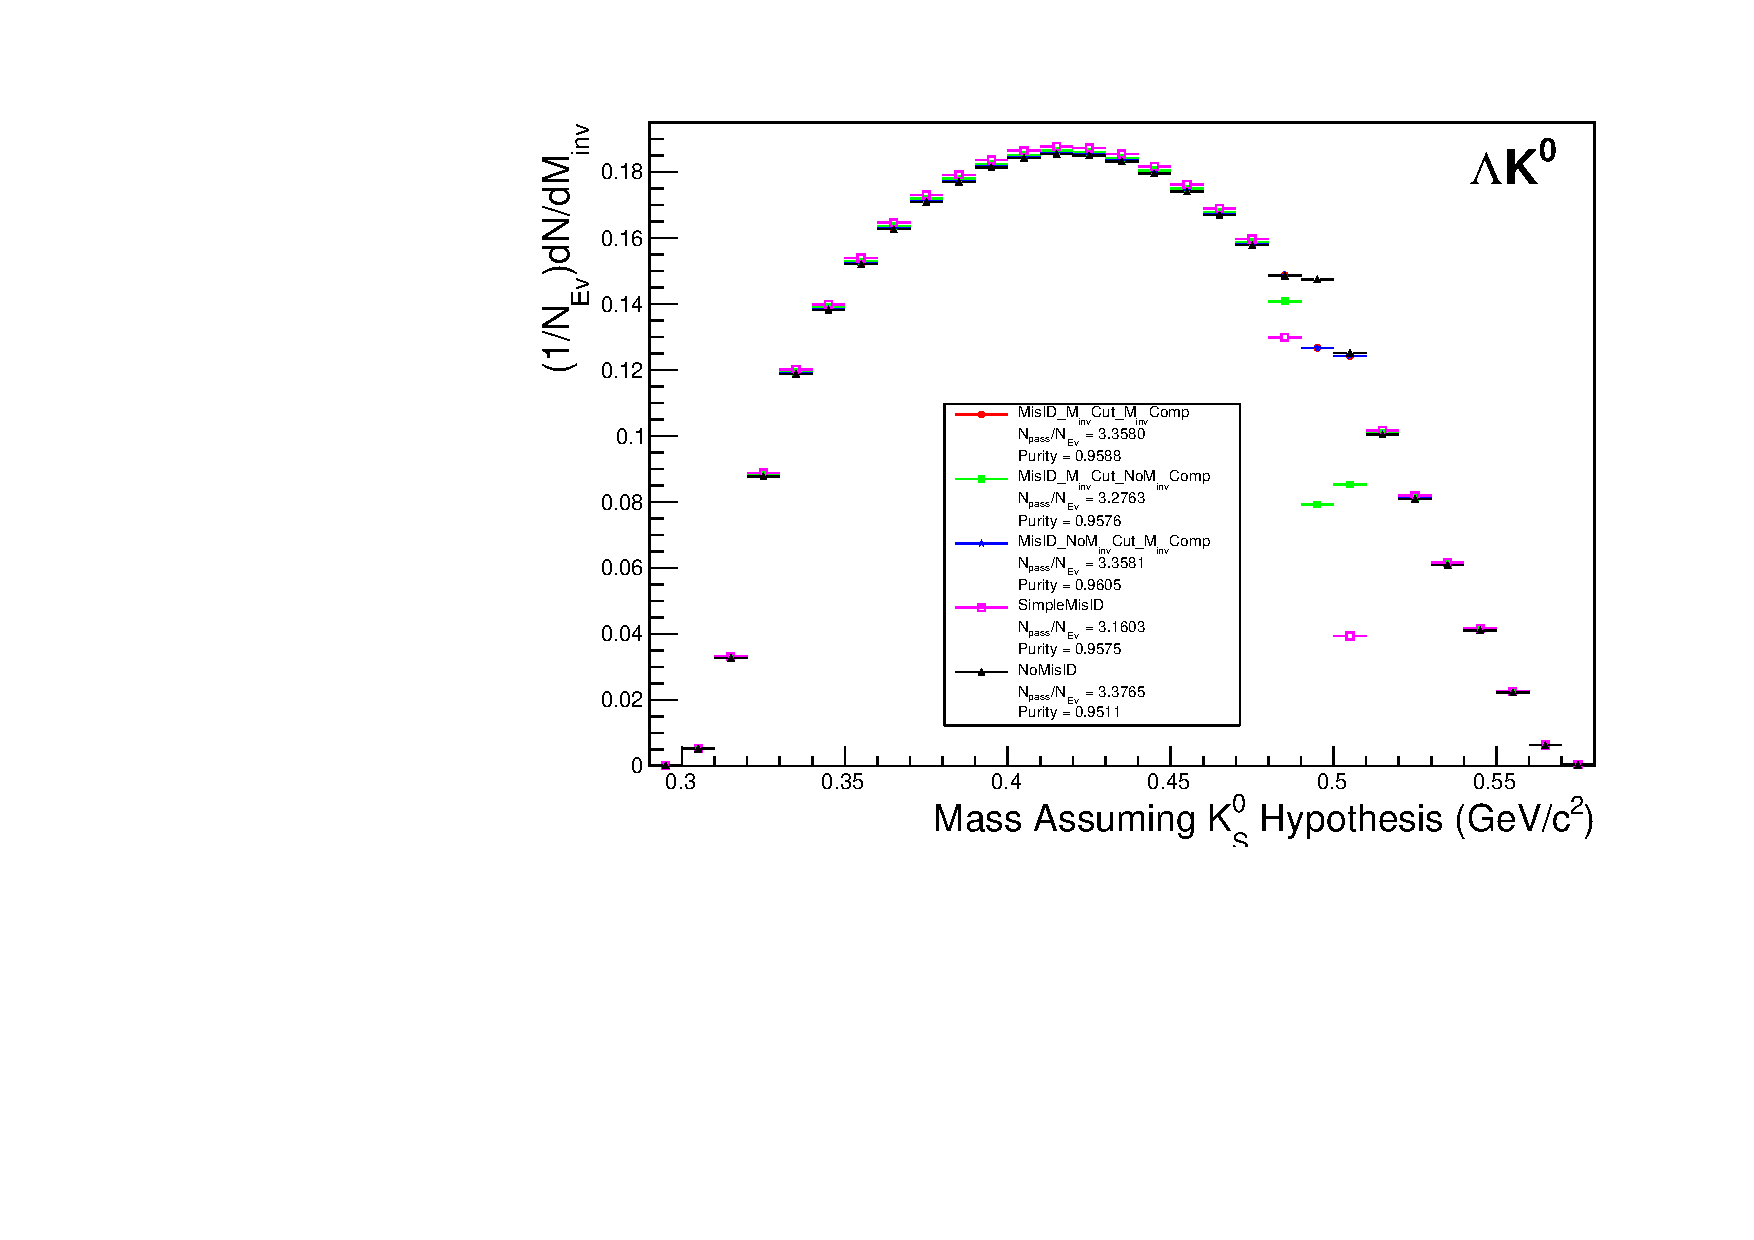
\includegraphics[width=0.49\textwidth]{3_DataSelection/Figures/MassAssHypotheses/canMassAssK0HypCompare_LamK0_wNoMisID.pdf}}%\\
  %%----start of second subfigure---
  \subfloat[Mass assuming K$^{0}_{S}$-hypothesis for $\bar{\Lambda}$ collection, \newline i.e. assume the daughters are $\pi^{+}\pi^{-}$ instead of $\pi^{+}\bar{p}^{-}$.]{
    \label{fig:MassAssK0ShortHyp_cLamK0:b}
    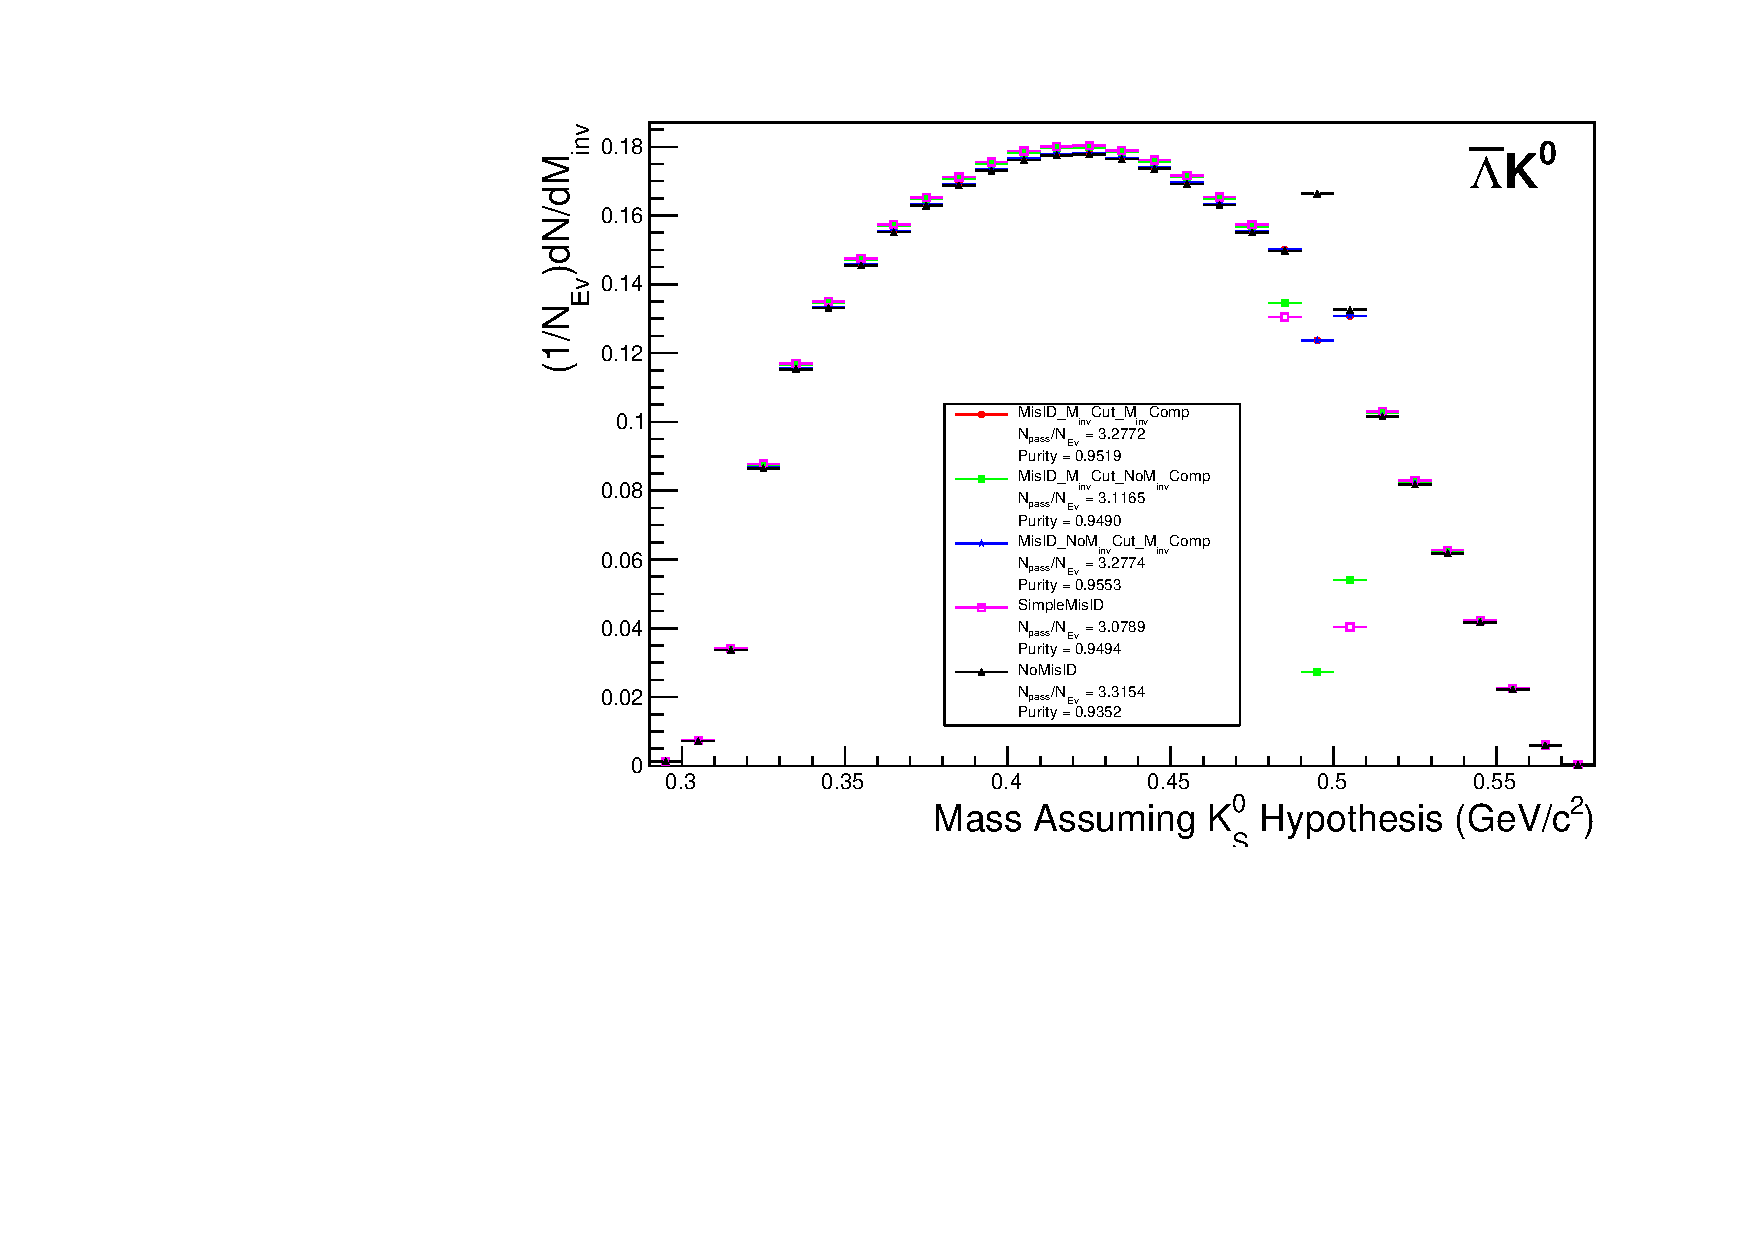
\includegraphics[width=0.49\textwidth]{3_DataSelection/Figures/MassAssHypotheses/canMassAssK0HypCompare_ALamK0_wNoMisID.pdf}}
  %%----overall caption----
  \caption[K$^{0}_{S}$ contamination in $\Lambda$($\bar{\Lambda}$) collection]{Mass assuming K$^{0}_{S}$-hypothesis for V0 candidates passing all $\Lambda$ (\ref{fig:MassAssK0ShortHyp_cLamK0:a}) and $\bar{\Lambda}$ (\ref{fig:MassAssK0ShortHyp_cLamK0:b}) cuts.
  The ``NoMisID" distribution (black triangles) uses the V0 finder without any attempt to remove misidentified K$^{0}_{S}$.
  The slight peak in the ``NoMisID" distribution around $m_{inv}$ = 0.5 GeV/c$^{2}$ likely contains misidentified K$^{0}_{S}$ particles in our $\Lambda$ collection.  
  ``SimpleMisID" (pink squares) simply cuts out the entire peak, which throws away some good $\Lambda$ and $\bar{\Lambda}$ particles.
  ``MisID\_NoM$_{inv}$Comp" (green squares) uses the misidentification cut outlined in the text, but does not utilize the invariant mass comparison method.
  ``MisID\_M$_{inv}$Comp" (red circles) utilizes the full misidentification methods, and is currently used for this analysis.  
  ``N$_{pass}$/N$_{ev}$" is the total number of $\Lambda$($\bar{\Lambda}$) particles found, normalized by the total number of events.  The purity of the collection is also listed.   
If one simply cuts out the entire peak, good $\Lambda$ particles will be lost.
Ideally, the $\Lambda$ selection and K$^{0}_{S}$ misidentification cuts are selected such that the peak is removed from this plot while leaving the distribution continuous.}
  \label{fig:MassAssK0ShortHyp_cLamK0}
\end{figure}


\begin{figure}[h!]
  \centering
  %%----start of first subfigure---  
  \subfloat[$\Lambda$ Purity]{
    \label{fig:cLamPurity:a}
    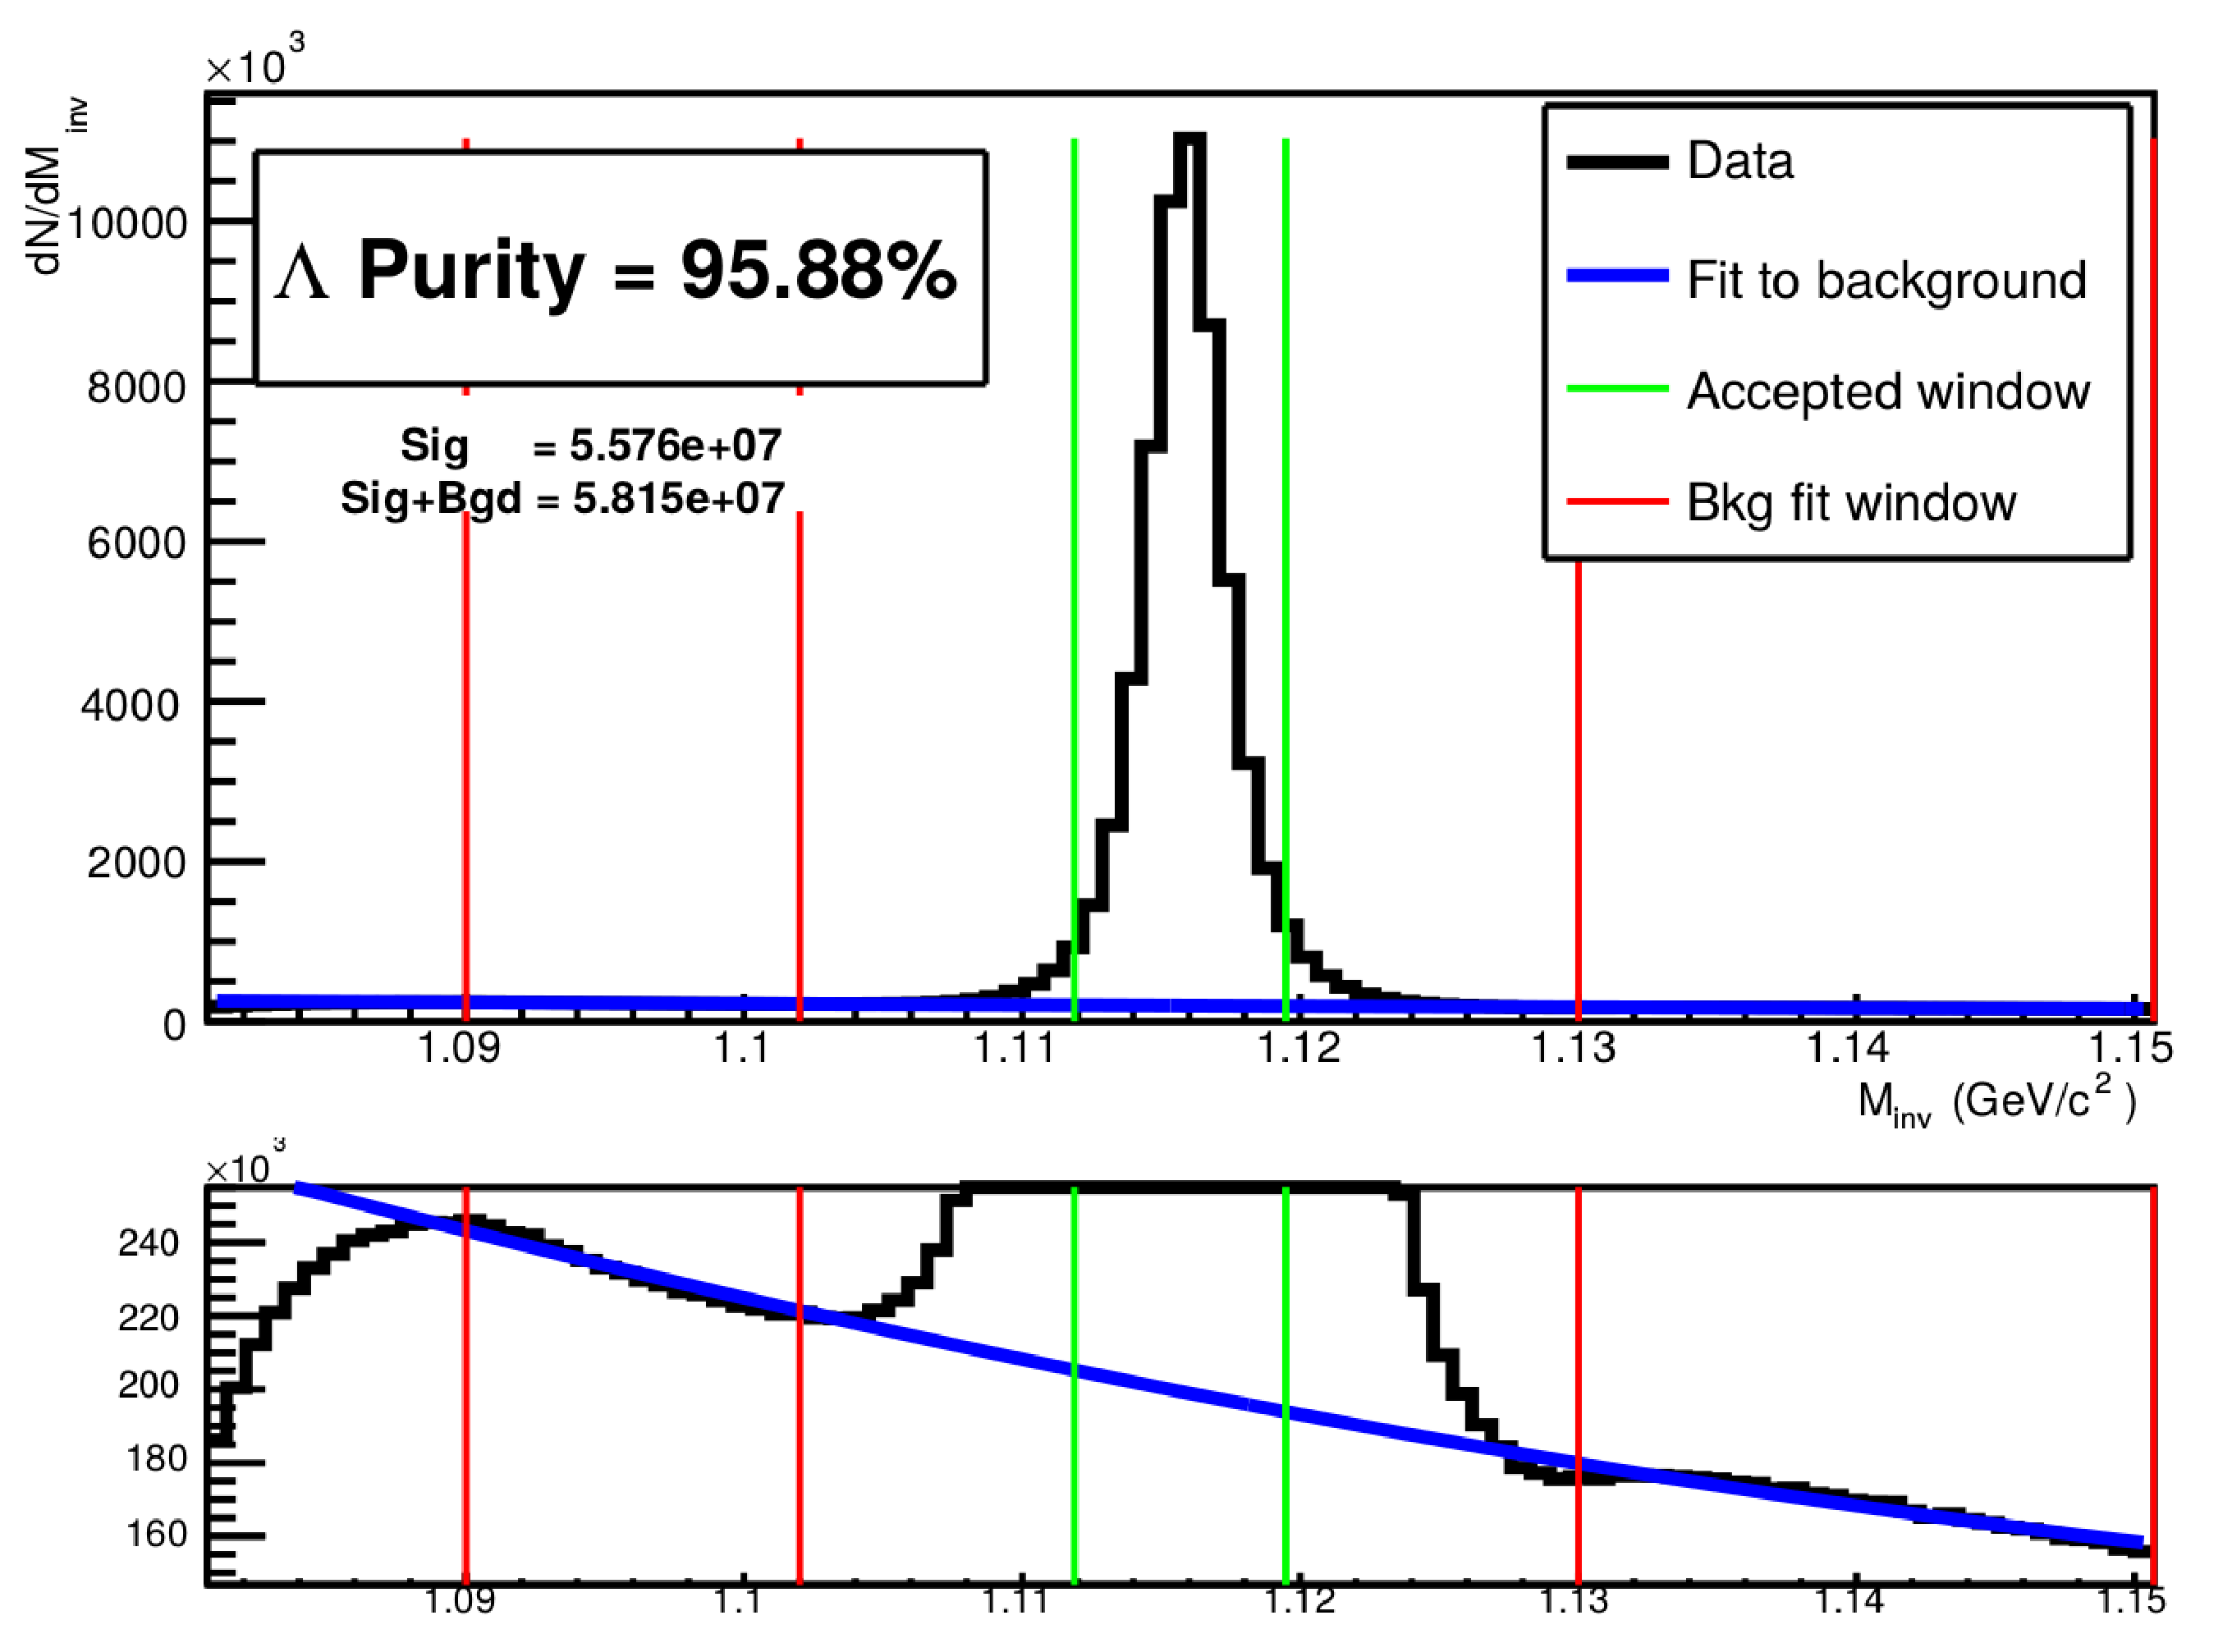
\includegraphics[width=0.49\textwidth]{3_DataSelection/Figures/LamPurity_LamKch_0010.pdf}}%\\
  %%----start of second subfigure---
  \subfloat[$\bar{\Lambda}$ Purity]{
    \label{fig:cLamPurity:b}
    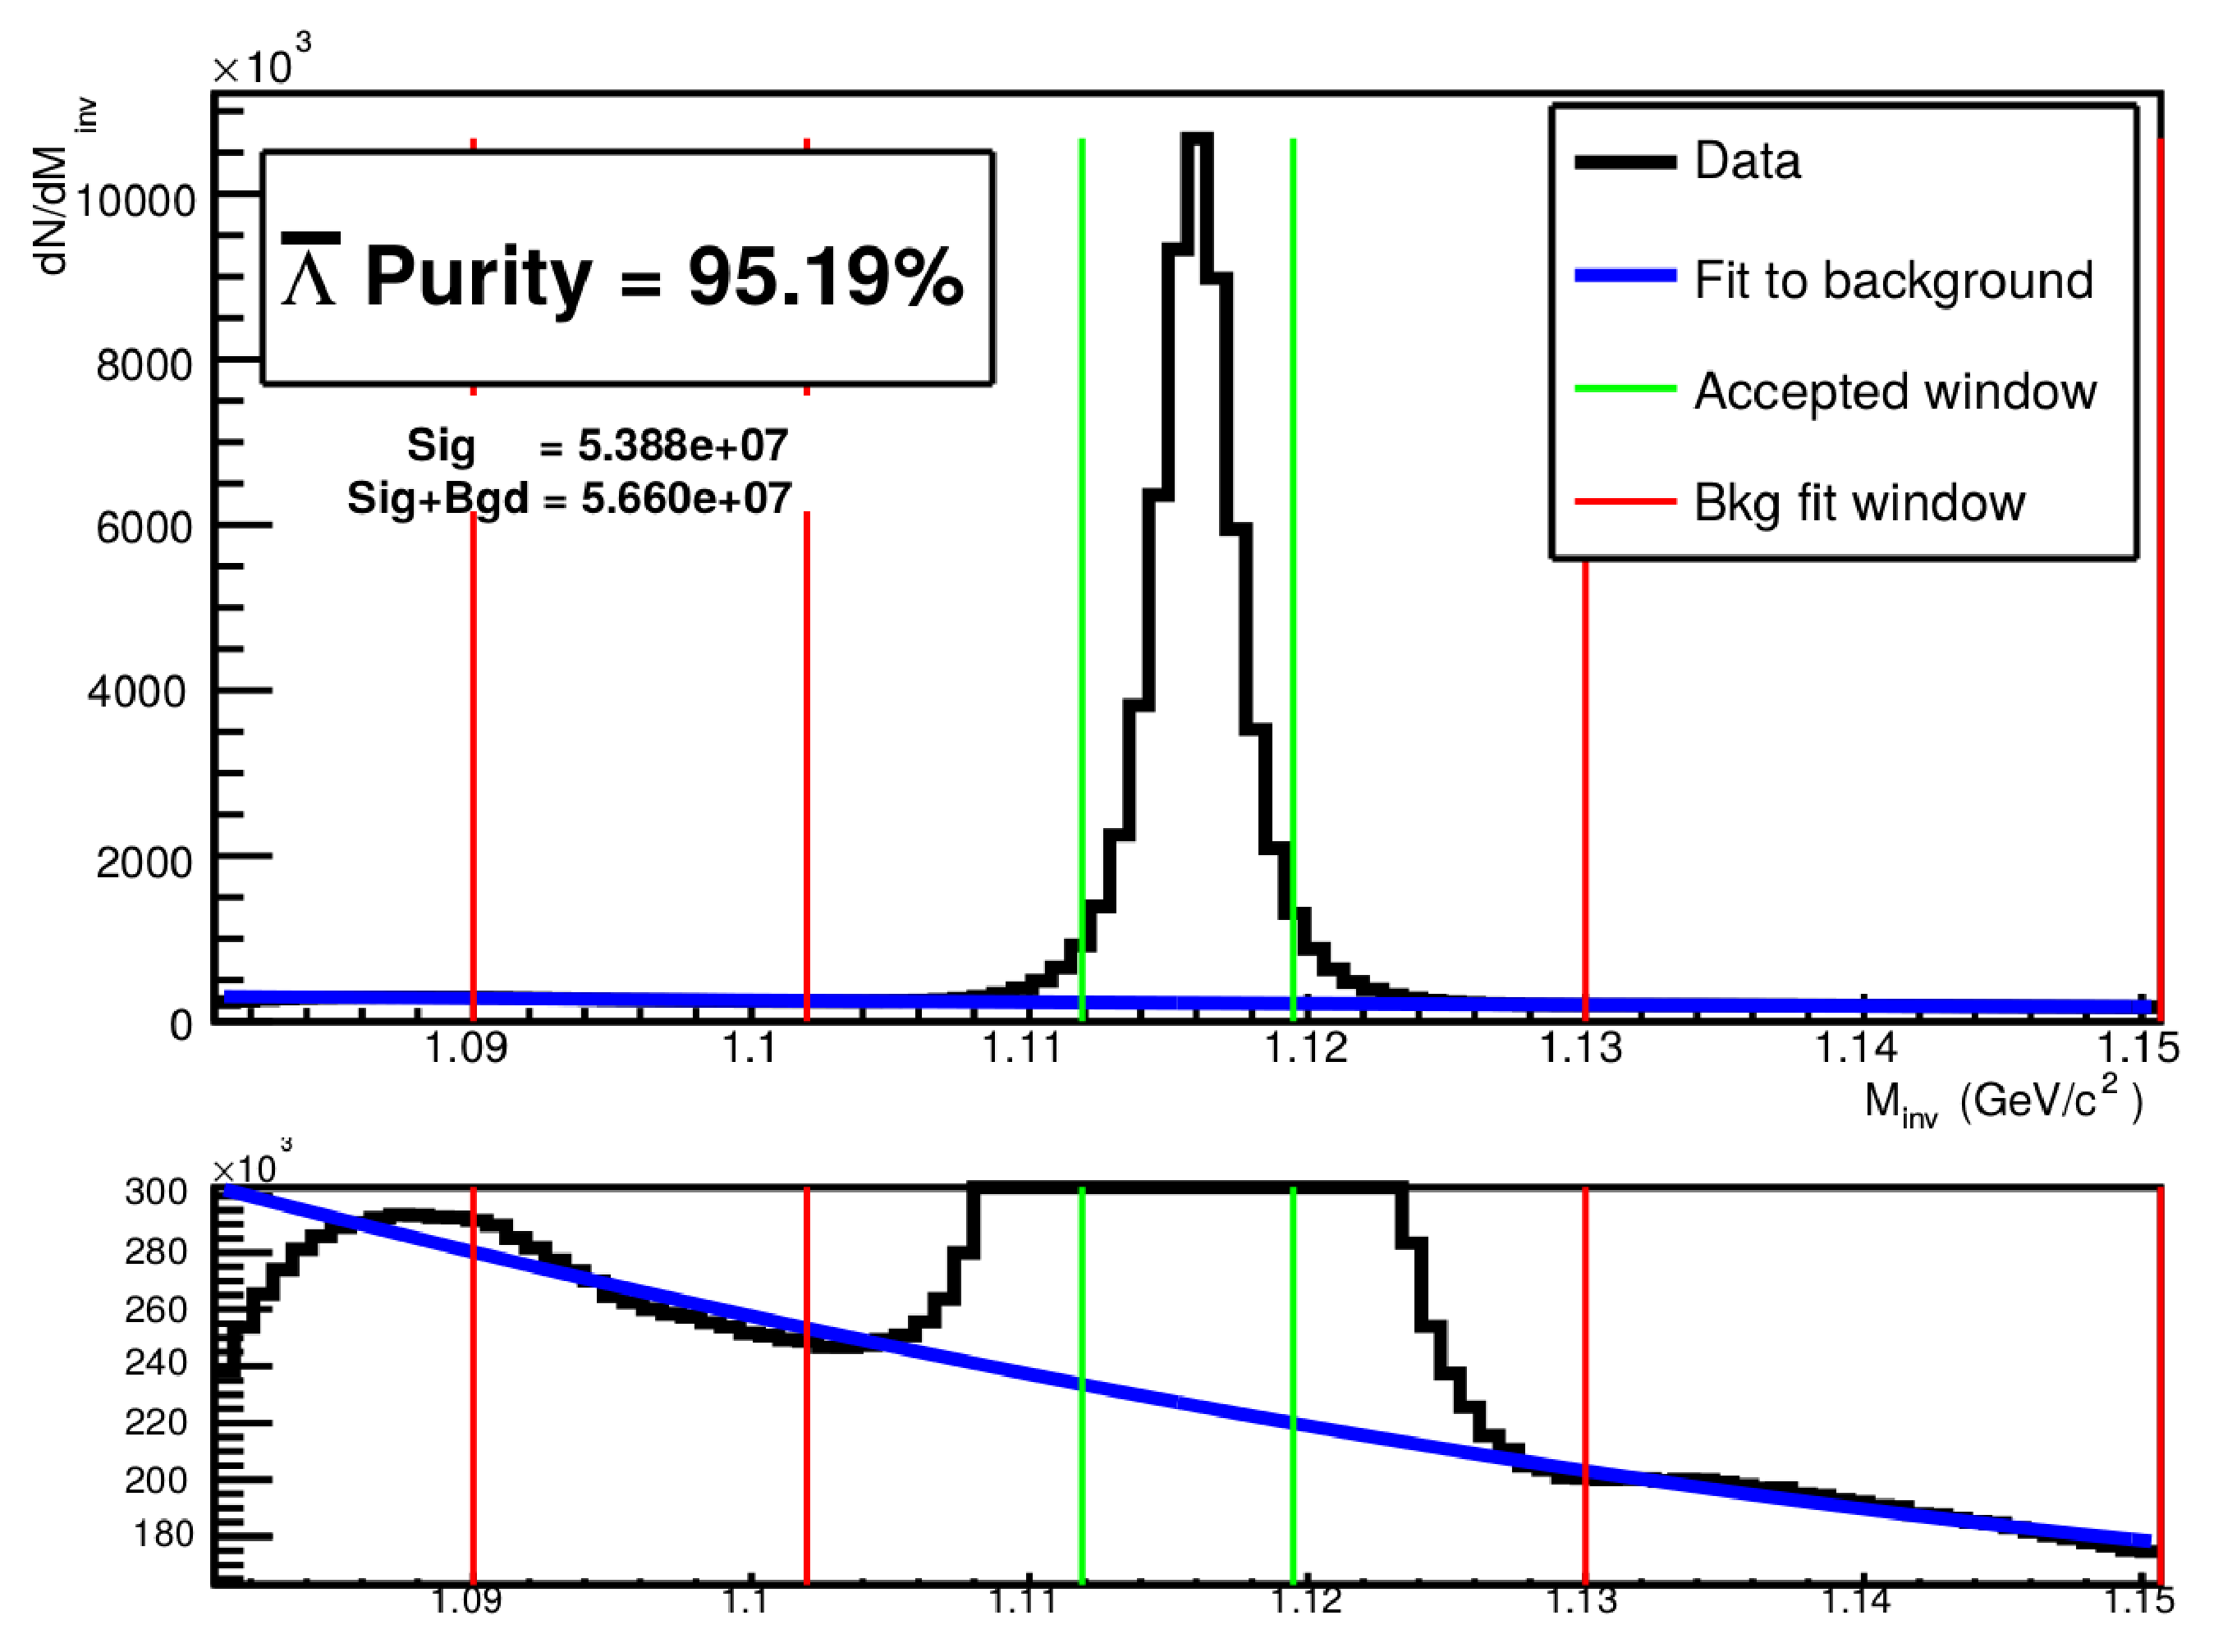
\includegraphics[width=0.49\textwidth]{3_DataSelection/Figures/ALamPurity_LamKch_0010.pdf}}
  %%----overall caption----
  \caption[$\Lambda$ and $\bar{\Lambda}$ Purity]{$\Lambda$ and $\bar{\Lambda}$ Purity}
  \label{fig:cLamPurity}
\end{figure}

\end{document}